\documentclass[11pt]{standalone}
%\usetheme{simple}
% \setbeamertemplate{footline}{} 
\usepackage{tikz, pgfplots,amsmath, amssymb, amsthm}   
\usepgfplotslibrary{groupplots}

\usepackage{sansmathaccent}
\pdfmapfile{+sansmathaccent.map}


%\pgfplotsset{ every non boxed y axis/.append style={y axis line style=-}}
% \setbeamertemplate{navigation symbols}{}
\begin{document}

  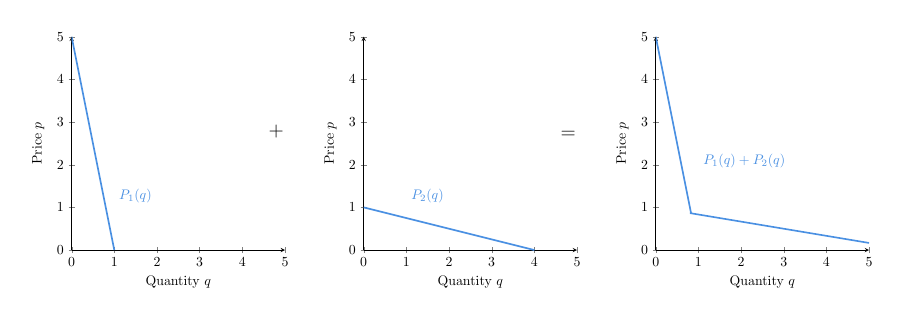
\begin{tikzpicture}[scale=.5]
    \begin{groupplot}[
      group style={group size=3 by 1, horizontal sep=2cm}, no markers,
      height=7cm, width=7cm,
      axis x line=bottom, axis y line=left,
      ymin=0, ymax=24,
      extra y ticks={23},  extra y tick labels={$\mathbf{E}\{R\}$},
    extra y tick style={major tick length=0mm, grid=none},
    scatter/classes={
      a={mark=o,draw=black, mark size = 3pt},
      b={mark=*, mark size = 3pt,draw=red, fill = red},
      c={mark=*, mark size = 3pt,draw=black, fill = black}
    }
]
% PLOT 1
\nextgroupplot[
   ylabel = Price $p$, xlabel = Quantity $q$,
  ymin=0, ymax=5, xmin=0, xmax=5,
  extra x tick style={major tick length=0mm, grid=none},
  extra y tick style={major tick length=0mm,  grid=none},
]
    
\addplot[scatter,only marks, scatter src=explicit symbolic]
  coordinates {(20, 11) (12, 5) };

\node at (axis cs:12, 5) [anchor=south west] {A};
\node at (axis cs:20,11) [anchor=north west] {B};
\addplot[color={rgb, 255:red, 74; green, 144; blue, 226 }, very thick,  domain=0:1, samples=1000, variable=\t]({t},  {5-5*t} );
\node at (axis cs:4.5, 2.5) [anchor=south west] {\Large +};

\node[color={rgb, 255:red, 74; green, 144; blue, 226 }] at (axis cs:1,1) [anchor= south west] {$P_1(q)$};


  % PLOT 2
\nextgroupplot[
   ylabel = Price $p$, xlabel = Quantity $q$,
  ymin=0, ymax=5, xmin=0, xmax=5,
  extra x tick style={major tick length=0mm, grid=none},
  extra y tick style={major tick length=0mm,  grid=none},
]
    
\addplot[scatter,only marks, scatter src=explicit symbolic]
  coordinates {(20, 11) (12, 5) };
\node at (axis cs:4.5, 2.5) [anchor=south west] {\Large=};

\node at (axis cs:20,11) [anchor=north west] {B};
\addplot[color={rgb, 255:red, 74; green, 144; blue, 226 }, very thick,  domain=0:4, samples=1000, variable=\t]({t},  {1-t/4} );


\node[color={rgb, 255:red, 74; green, 144; blue, 226 }] at (axis cs:1,1) [anchor= south west] {$P_2(q)$};

   % PLOT 3
\nextgroupplot[
   ylabel = Price $p$, xlabel = Quantity $q$,
  ymin=0, ymax=5, xmin=0, xmax=5,
  extra x tick style={major tick length=0mm, grid=none},
  extra y tick style={major tick length=0mm,  grid=none},
]
    
\addplot[scatter,only marks, scatter src=explicit symbolic]
  coordinates {(20, 11) (12, 5) };

\node at (axis cs:12, 5) [anchor=south west] {A};
\node at (axis cs:20,11) [anchor=north west] {B};
\addplot[color={rgb, 255:red, 74; green, 144; blue, 226 }, very thick,  domain=0:0.83, samples=1000, variable=\t]({t},  {5-5*t} );
\addplot[color={rgb, 255:red, 74; green, 144; blue, 226 }, very thick,  domain=0.8:5, samples=1000, variable=\t]({t},  {1-t/6} );


\node[color={rgb, 255:red, 74; green, 144; blue, 226 }] at (axis cs:1,1.8) [anchor= south west] {$P_1(q)+P_2(q)$};

  \end{groupplot}

  
  
 
%   \draw[dashed] (ko1) -- (ko2) ;
%   \draw[dashed] (ms1) -- (ms2) ;
 \end{tikzpicture}

\end{document}